\documentclass[letterpaper,11pt]{article}
\oddsidemargin -1.0cm \textwidth 17.5cm

\usepackage[utf8]{inputenc}
\usepackage[activeacute,spanish]{babel}
\usepackage{amsfonts,setspace}
\usepackage{amsmath}
\usepackage{amssymb, amsmath, amsthm}
\usepackage{comment}
\usepackage{float}
\usepackage{amssymb}
\usepackage{dsfont}
\usepackage{anysize}
\usepackage{multicol}
\usepackage{enumerate}
\usepackage{graphicx}
\usepackage[left=1.5cm,top=1.5cm,right=1.5cm, bottom=1.7cm]{geometry}
\setlength\headheight{1.5em} 
\usepackage{fancyhdr}
\usepackage{multicol}
\usepackage{hyperref}
\usepackage{wrapfig}
\usepackage{subcaption}
\pagestyle{fancy}
\fancyhf{}
\renewcommand{\labelenumi}{\normalsize\bfseries P\arabic{enumi}.}
\renewcommand{\labelenumii}{\normalsize\bfseries (\alph{enumii})}
\renewcommand{\labelenumiii}{\normalsize\bfseries \roman{enumiii})}

\begin{document}

\fancyhead[L]{\itshape{Facultad de Ciencias F\'isicas y Matem\'aticas}}
\fancyhead[R]{\itshape{Universidad de Chile}}

\begin{minipage}{11.5cm}
    \begin{flushleft}
        \hspace*{-0.6cm}\textbf{FI1100-6 Introducción a la Física Moderna}\\
        \hspace*{-0.6cm}\textbf{Profesor:} Diego Mardones\\
        \hspace*{-0.6cm}\textbf{Auxiliares:} Gabriel O\textsc{\char13}Ryan, Camila Sepúlveda, Alejandro Silva\\
        \hspace*{-0.6cm}\textbf{Ayudante:} Sebastián Vargas
    \end{flushleft}
\end{minipage}

\begin{picture}(2,3)
    \put(366, 10){
\includegraphics[scale=0.9]{Imágenes/logo/dfi-fcfm.pdf}}
\end{picture}

\begin{center}
	\LARGE\textbf{Auxiliar 3 }\\
	\Large{Ondas}
\end{center}

\vspace{-1cm}
\begin{enumerate}\setlength{\itemsep}{0.4cm}

\rfoot[]{pág. \thepage}

\item[]

\item Se tiene una cuerda de densidad $\rho$ bajo una tensión T, donde en el punto $x=0$ se le coloca una masa m. Considere que la masa solo tiene movimiento vertical y que no hay gravedad.\\
Se acerca una onda con forma $A cos(kx-wt)$ desde el lado izquierdo:
    \begin{enumerate}
         \item Describa como será la forma de las ondas transmitidas y reflejadas. \\
         
        \item Escriba las condiciones de borde para la onda y DCL para la masa.  \\

        \item Encuentre las ondas transmitidas y reflejados por la masa en función de la onda inicial. \\

        \item Considere casos límites para la masa m, comente como se comporta la transmisión y reflexión ¿tiene sentido?.\\
        
        \item Calcule la potencia generada por la cuerda y comente para los casos limites. \\

        \item ¿Como cambiaría el comportamiento de las ondas si la masa estuviera bajo fuerzas externas, por ej: la gravedad o unida a un resorte de constante elástica $\kappa$ y largo natural en y=0?. Calcule y comente para estos casos, en especial analice como depende la transmisión de $\kappa$.
        
    \end{enumerate}
    
    \begin{figure}[h]
        \centering
        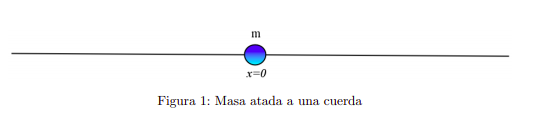
\includegraphics[0.2=\textwidth]{Imágenes/aux3/cuerda.png}
        \label{fig:my_label}
    \end{figure}
    
    \item  Ahora considere una cuerda con las mismas variables anteriores (pero sin la masa), que posee una densidad $\lambda$ distinta a $\rho$ entre x=0 y x=L.
   \begin{enumerate}
       \item  Imponiendo las condiciones de borde correctas, encuentre la forma de los pulsos en las 3 zonas de la cuerda.
        \item Por último imponga el límite que L tienda a cero y use que $\lambda L=m$ en este límite. ¿Como es el resultado en las ondas transmitidas y reflejadas? Compare con la P1
   \end{enumerate}
        

\end{enumerate}
\end{document}